\documentclass[conference]{IEEEtran}
\usepackage{blindtext, graphicx}
\usepackage{amssymb}
\usepackage{multirow}
\usepackage[table,xcdraw]{xcolor}
\usepackage{cite}

%%%%%%%%%%%%%%%%%%%%%%%%%%%%%%%%%%%%%%%%%%%%%%%%%%%%%%%%%%%%%%%%%%%%%
%%%  Used packages
%%%%%%%%%%%%%%%%%%%%%%%%%%%%%%%%%%%%%%%%%%%%%%%%%%%%%%%%%%%%%%%%%%%%%
\usepackage{amsmath}
\usepackage{amssymb}
% \usepackage{amsthm}
\usepackage{mathtools}                      % \mathrlap
\usepackage{stmaryrd}                       % double square brackets
\usepackage{cancel}                         % \notModels
\usepackage{xspace}                         % macros followed by a space
\usepackage[inline,nomargin]{fixme}         % Notes on things yet to do.
\usepackage{float}                          % More placement control on floats
\usepackage{fancyhdr}                       % Custom page headers
\usepackage{graphicx}
\usepackage{xcolor}
\usepackage{microtype}
\usepackage{algorithmic}
\usepackage[normalem]{ulem}                 % underline text using \uline
\usepackage{ragged2e}

\usepackage{pgf,tikz}
\usetikzlibrary{shapes,patterns,calc,through,arrows,positioning,matrix,trees,fit,petri,fadings,shadows,decorations.pathreplacing}
%\usetikzlibrary{shapes,patterns,calc,through,arrows,positioning,matrix,trees,fit,petri,fadings,shadows}
\pgfdeclarelayer{background}
\pgfsetlayers{background,main}

\usepackage{array,booktabs}
\usepackage{listings}
\usepackage[utf8]{inputenc}

%% Better TT fonts!
\usepackage[scaled=.83]{beramono}           % nicer tt font
\usepackage[T1]{fontenc}                    % otherwise beramono does not work

% \usepackage{csquotes}
% \addbibresource[label=bibliography]{radu.bib}

\usepackage{pdfsync}                        % for PDF viewer synchronisation
\usepackage{hyperref}
\usepackage{float}                          % \begin{figure}[H] ...
\usepackage{cite}
\usepackage{epstopdf}


%%%%%%%%%%%%%%%%%%%%%%%%%%%%%%%%%%%%%%%%%%%%%%%%%%%%%%%%%%%%%%%%%%%%%
%%%  Common HATS definitions
%%%%%%%%%%%%%%%%%%%%%%%%%%%%%%%%%%%%%%%%%%%%%%%%%%%%%%%%%%%%%%%%%%%%%

\definecolor{darkblue}{rgb}{0,0,0.6}
\definecolor{darkgreen}{rgb}{0,0.6,0}
\definecolor{darkred}{rgb}{0.7,0,0}
\definecolor{orange}{rgb}{1,0.5,0}
\newcommand{\Black}[1]{\color{black}#1\color{black}}
\newcommand{\White}[1]{\color{white}#1\color{black}}
\newcommand{\Red}[1]{\color{red}#1\color{black}}
\newcommand{\Purple}[1]{\color{purple}#1\color{black}}
\newcommand{\Green}[1]{\color{darkgreen}#1\color{black}}
\newcommand{\Gray}[1]{\color{gray}#1\color{black}}
\newcommand{\Blue}[1]{\color{blue}#1\color{black}}


% handy notes to mark work-in-progress, TODOs etc.
\newcommand{\mynote}[1]{
  \ensuremath{\left\langle\right.\!\!\left\langle\right.\!}\bf #1%
  \ensuremath{\!\left.\right\rangle\!\!\left.\right\rangle}}
% \newcommand{\DC}[1]{\textcolor{blue}{\mynote{DC: #1}}}
\newcommand{\MR}[1]{\textcolor{darkred}{\mynote{Maya: #1}}} % Maya
\newcommand{\RM}[1]{\textcolor{darkgreen}{\mynote{Radu: #1}}} % Radu
%\renewcommand{\mynote}[1]{}

\newcommand{\wrap}[1]{\begin{tabular}{@{}c@{}}#1\end{tabular}}
\newcommand{\wrapl}[1]{\begin{tabular}{@{}l@{}}#1\end{tabular}}

% highlight code
% usage example: $\cbox{getProduct}$
\newcommand{\cbox}[2][2.6pt]{\raisebox{-#1}{\tikz{\node[inner sep=1.2pt,fill=yellow!70] {#2};}}}

\definecolor{hlcolor}{rgb}{1,0.5,0.5}
\newcommand{\hlbox}[1]{\colorbox{hlcolor}{#1}}
\newcommand{\cfbox}[2]{%
    \colorlet{currentcolor}{.}%
    {\color{#1}%
    \fbox{\color{currentcolor}#2}}%
}

% faded scope (use inside a tikzpicture)
\definecolor{faded}{rgb}{.5,.5,.5}
\newenvironment{faded}[1][faded]
    {   \pgfonlayer{background}
        \begin{scope}[#1]
        \def \Ucolor {#1}
        \def \ACcolor {#1}
        \tikzset{token/.append style={#1}}}
    {   \end{scope}
        \endpgfonlayer}


\colorlet{keywordcolor}{blue!50!black}
\colorlet{typecolor}{violet}
\newcommand{\sourcefont}{\ttfamily\small}
%\newcommand{\commentfont}{\slshape\rmfamily\color{black!70}}
\newcommand{\commentfont}{\slshape\rmfamily\color{green!70!black}}
%\renewcommand{\commentfont}{\slshape\color{black!70}}

%%%%%%%%%%%%%%%%%%%%%%%%%%%%%%%%%%%%%%%%%%%%%%%%%%%%%%%%%%%%%%%%%%%%%%%%%%%%%%%
%% ABS and Java code examples
%%%%%%%%%%%%%%%%%%%%%%%%%%%%%%%%%%%%%%%%%%%%%%%%%%%%%%%%%%%%%%%%%%%%%%%%%%%%%%%

\lstdefinelanguage{ABS}{
    keywords={assert,this,new,data,type,def,case,of,cog,class,interface,
    extends,implements,if,then,else,await,get,Fut,return,skip,while,module,
    import,export,from,to,suspend,delta,adds,modifies,removes,original,productline,
    features,core,corefeatures,optionalfeatures,after,when,product,hasAttribute,
    hasMethod,hasField,hasInterface,uses,root,extension,group,allof,oneof,require,
    stateupdate,objectupdate,classupdate,
    exclude,original,ifin,ifout,opt,null,%critical,port,rebind,duration,deadline,now,
    newgroup,data,thiscomp,in,joins,leaves,subtypeOf,wait,acquire,except,as,component,Pre,Abs
    },
    keywordstyle=\color{keywordcolor}\bf\sffamily,
    % standard types:
    morekeywords=[2]{Unit, Int, Bool, Rat, List, Set, Pair, Fut, Maybe, String, Triple, Either, Map},
    keywordstyle=[2]\color{typecolor},
    sensitive=true,
    comment=[l]{//},
    morecomment=[s]{/*}{*/},
    morestring=[b]",
    numbers=left,
    numberstyle=\tiny
}

% Java 9 dialect
\lstdefinelanguage[v9]{Java}[]{Java}{
    morekeywords={module,requires,provides,with,exports,local,optional,service}
}
% ContextJ dialect
\lstdefinelanguage[ContextJ]{Java}[]{Java}{
    morekeywords={layer,with,without,proceed,before,after}
}
% FOP dialect
\lstdefinelanguage[FOP]{Java}[]{Java}{
    morekeywords={refines,original,Super}
}

\lstdefinestyle{code}{
    basicstyle=\sourcefont\upshape,
    keywordstyle=\color{keywordcolor}\bf\sffamily,
    commentstyle=\commentfont,
    classoffset=1,
    classoffset=0,
    columns=fullflexible,
    mathescape=false,
    showstringspaces=false,
    inputencoding=utf8,
    extendedchars,
    xleftmargin=4pt,
    aboveskip=8pt, % default is \medskipamount
    xrightmargin=4pt,
    numberstyle=\ttfamily\scriptsize\color{gray},stepnumber=1, numbersep=8pt,
}

\lstdefinestyle{XXXXX}{
    style=code,
    language=ABS,
}


\lstdefinestyle{abs}{
    style=code,
    language=ABS,
}
\lstdefinestyle{java}{
    style=code,
    language=Java
}
\lstdefinestyle{java9}{
    style=code,
    language=[v9]Java
}
\lstdefinestyle{aspectj}{
    style=code,
    language=[AspectJ]Java
}
\lstdefinestyle{contextj}{
    style=code,
    language=[ContextJ]Java
}
\lstdefinestyle{FOP}{
    style=code,
    language=[FOP]Java
}
\lstdefinestyle{scala}{
    style=code,
    language=Scala,
    morekeywords={self}
}

\newcommand{\code}[2][]{\lstinline[style=code,basicstyle=\ttfamily\upshape,#1]{#2}}
\newcommand{\java}[2][]{\code[style=java,#1]{#2}}
\newcommand{\abs}[2][]{\code[style=abs,#1]{#2}}
\newcommand{\scala}[2][]{\code[style=scala,#1]{#2}}

\lstnewenvironment{srccode}[1][]{
    \minipage{\linewidth}
    \lstset{style=code,
    %framerule=1pt,
    backgroundcolor=\color{white},
    rulecolor=\color{gray!50},
    frame=tblr,
    captionpos=b,
    #1}
}{\endminipage}

\lstnewenvironment{abscode}[1][]{
    \minipage{\linewidth}
    \lstset{style=abs,
    %framerule=1pt,
    backgroundcolor=\color{white},
    rulecolor=\color{gray!50},
    frame=tblr,
    captionpos=b,
    #1}
}{\endminipage}

\lstnewenvironment{javacode}[1][]{
    \minipage{\linewidth}
    \lstset{style=java,
    %framerule=1pt,
    backgroundcolor=\color{gray!5},
    rulecolor=\color{gray!50},
    frame=tblr,
    captionpos=b,
    #1}
}{\endminipage}




\hyphenation{op-tical net-works semi-conduc-tor}


\begin{document}
%
% paper title
\title{Object-Relational Mapping \\of Software Product Lines in the ABS Language}


% author names and affiliations
\author{\IEEEauthorblockN{Niken Fitria Apriani and Ade Azurat}
\IEEEauthorblockA{Faculty of Computer Science\\
Universitas Indonesia\\
Depok, Indonesia}
\and
\IEEEauthorblockN{Radu Muschevici}
\IEEEauthorblockA{Fachbereich Informatik\\
Technische Universitat Darmstadt\\
Darmstadt, Germany}}


\maketitle


\begin{abstract}

Software Product Lines (SPL) employ variability modelling to ease development of
software products that are tailored to variable customer requirements.
% If these
% products use a relational database, the corresponding database schema needs
% to be adapted according to variability of the application's data storage model.
The data storage models of the individual products can vary according to the
chosen features of each product. It is therefore desirable to include
data storage variability in the overall variability model of the SPL.
%
When the data is stored in a relational database, the variability model of the
SPL needs to account for variability in the design and implementation of the
database schema. For this purpose, we devise a technique to control the
variability of the database schema from within the SPL. This technique consists
of building an object model of the database, and a set of mapping rules to the
relational model. We implement our technique as part of the Abstract Behavioral
Specification (ABS) language, a delta-oriented modelling language equipped for
SPL engineering.
%
By modelling the variability of the relational database schema,
the appropriate database schema for each product of the SPL can be generated automatically.
Consequently, requirement changes that alter the feature composition of a
product will adjust the database schema accordingly. This eliminates potential
incompatibility between application logic and data storage model.



% Feature variability of an application in Software Product Lines (SPL) can
% affect the design and the implementation of database schema of the application,
% if the feature is related to the data storage of the application.
%
% However, this
% crucial thing is not handled by the management technique of variability in SPL,
% hence this can make database schema inconsistent and incompatible with the
% application requirements. This study shows delta modeling in ABS (Abstract
% Behavioral Specification) is able to adjust database schema based on requirement
% changes to realize feature variance. To this end, we develop mapping mechanism
% of delta modeling in ABS into relational database schema. By integrating the
% mapping technique with existing ABS Tools, the appropriate database schema for
% each product of the SPL can be generated.

\end{abstract}

\begin{IEEEkeywords}
ORM, ABS, delta modeling, delta, core, relational database, database schema, constraints
\end{IEEEkeywords}


\section{Introduction}
The development of software engineering cannot be separated from the influence of market and industry demand. The development of market and industry nowadays demand for software which has variability be suited with the choice and the need of the users. This could cause repeated requirement changes for the same kind of software or system.

The problem above actually has been addressed by a methodological approach called SPL (Software Product Line). Software product line (SPL), is a methodology for developing diversed software products and software-intensive systems. According to \cite{book1}, SPL can be used to develop software products with diversity at lower cost, in shorter time, and with high quality, compared to single product development methodology.

ABS (Abstract Behavioral Specification) is a modeling language which supports SPL methodology \cite{lncschap}. In SPL software variability is commonly expressed using features, and in ABS these features are organized in feature model to express the dependencies between features \cite{url}. Moreover, ABS also applies delta modeling to handle requirement changes in the process of feature adjustment, which is by implementing changes without changing the default system.

Many software application relies on database to manage data, therefore database is an important element of software system. Furthermore database is also influenced by requirement changes resulted by SPL implementation. In SPL, the variability of software, information system for example, will cause variability in database schema and database implementation. Until now, there is no technique in SPL methodology to manage variability in database schema and database implementation, especially in information system \cite{article}. This paper is concerned in applying delta modeling in ABS to not only influence and adjust the  SPL implementation, but also the changes of database schema.

The main contribution of this paper is the mapping technique of delta modeling in ABS into relational database schema. The follows are the organizations of this paper.
The first section is the introduction of the paper.
Section two discusses about the mapping technique from delta oriented programming into relational database introduced by this paper.
The last section provides the conclusion and the future work of this research.

\section{Mapping Technique}
This section describes the proposed mapping technique used in the mapping process from ABS code into relational database schema. The mapping technique is defined based on relational database schema and the basic syntax of ABS modules. This section is divided into several parts as follows:
\begin{enumerate}
	\item The steps used in defining the mapping technique
	\item The elements of relational database schema as the target of the mapping
	\item The mapping of core ABS component and delta module into relational database schema elements
	\item The mismatch between ABS language and relational database schema and the solution for it
\end{enumerate}

\subsection{The Methodology of Mapping Technique}
ORM(Object Relational Mapping) does the mapping works between object model in object oriented programming and relational model in relational database. There are three type of perspective used by ORM to do the mapping, those are:
\begin{enumerate}
	\item Metadata-oriented, which uses metadata as the input to generate the mapping code
	\item Application-oriented, which starts from object-oriented application to do the mapping
	\item Database-oriented, which does the mapping from the database.
\end{enumerate}

The mapping technique proposed in this research uses the last perspective used by ORM, which is database-oriented approach. Hence the approach to do the mapping is started from the target of the mapping, which is the relational database schema. The following are the steps used in defining the mapping technique:

\begin{enumerate}
	\item Analyze the aspect of relational database schema\\
	In this step we obtain the elements of relational database schema and what is needed to create a relational database schema. Based on those elements, we define the information which needs to be provided by the ABS model so it can be generated into database schema.
	\item Analyze the components of ABS\\
	In this step we analyze the component of ABS modules and their syntax. Then we define the components which provide the information needed to create a relational database schema. After that, those components are mapped into the corresponding relational database schema’s elements.
	\item Analyze the mismatch between ABS language and relational database schema and define the solutions\\
	This step is done by revisiting step 1 and step 2. In this step we find the elements of relational database schema which are not provided by the ABS language. Furthermore, we also find the components of ABS modules which are not available in relational database concept. So we define the solution to the mismatch, by considering the constraints of each concept.
\end{enumerate}

\subsection{Relational Database Schema Elements}
The main elements of relational database schemes are tables and constraints \cite{book2}. Tabel I presents the components of a relational database schema.

\begin{table}[]
	\centering
	\caption{The Representation of Relational Database Schema Components}
	\label{tabel1}
	\begin{tabular}{|l|l|l|l|}
		\hline
		\multirow{9}{*}{schema} & \multirow{7}{*}{table} & \multirow{3}{*}{attribute}   & name              \\ \cline{4-4}
		&                        &                              & data type         \\ \cline{4-4}
		&                        &                              & {[}constraints{]} \\ \cline{3-4}
		&                        & \multicolumn{2}{c|}{\multirow{2}{*}{:}}          \\
		&                        & \multicolumn{2}{c|}{}                            \\ \cline{3-4}
		&                        & \multirow{2}{*}{constraints} & Primary Key       \\ \cline{4-4}
		&                        &                              & {[}Foreign Key{]} \\ \cline{2-4}
		& \multicolumn{3}{c|}{\multirow{2}{*}{:}}                                   \\
		& \multicolumn{3}{c|}{}                                                     \\ \hline
	\end{tabular}
\end{table}

In a database schema there will be at least one table. In each table, there will be at least one attribute, there must be one primary key, and there could be any number of foreign keys. In each attribute, there must be an attribute name, there must be an attribute data type, and there could be any attribute constraints. Hence, we should extract the ABS code to get the information about:
\begin{itemize}
	\item table(s)
	\begin{itemize}
		\item attribute(s)
		\begin{itemize}
			\item attribute name
			\item attribute data type
			\item attribute constraint(s)
		\end{itemize}
		\item primary key
		\item foreign key
	\end{itemize}
\end{itemize}

\subsection{Core ABS and Delta Modules}
In this section, we analyze the core modules of ABS to obtain the information needed to generate a database schema. However ABS implements delta-oriented programming. Hence, we should also consider the modification done by the delta modules which will affect the ABS core.

\subsubsection*{Core ABS Mapping}
Core ABS contains at least one module. In each module, there could be any import and export from other modules, any interface declarations, any class declarations, any data type declarations, any function declarations, and main block. For every declared interface, there could be any abstract method declarations. For every class, there could be any class parameters, any interfaces implemented, any fields, and any methods. For every class parameter, there must be a data type and a name. Whereas for every field in a class, there must be a data type and a name, and there could be an initial value.


\begin{table}[]
	\centering
	\caption{The Representation of Core ABS Components}
	\label{table2}
	\begin{tabular}{|l|l|l|l|l|}
		\hline
		\multirow{23}{*}{core} & \multirow{22}{*}{module} & \multicolumn{3}{l|}{export}                                             \\ \cline{3-5}
		&                          & \multicolumn{3}{l|}{import}                                             \\ \cline{3-5}
		&                          & \multirow{2}{*}{interface} & \multicolumn{2}{l|}{abstract method}       \\ \cline{4-5}
		&                          &                            & \multicolumn{2}{c|}{:}                     \\ \cline{3-5}
		&                          & \multicolumn{3}{c|}{:}                                                  \\ \cline{3-5}
		&                          & \multirow{11}{*}{class*}   & \multirow{2}{*}{parameter*}  & data type*  \\ \cline{5-5}
		&                          &                            &                              & name*       \\ \cline{4-5}
		&                          &                            & \multicolumn{2}{c|}{:}                     \\ \cline{4-5}
		&                          &                            & \multicolumn{2}{l|}{implemented interface} \\ \cline{4-5}
		&                          &                            & \multicolumn{2}{c|}{:}                     \\ \cline{4-5}
		&                          &                            & \multirow{3}{*}{field*}      & data type*  \\ \cline{5-5}
		&                          &                            &                              & name*       \\ \cline{5-5}
		&                          &                            &                              & value*      \\ \cline{4-5}
		&                          &                            & \multicolumn{2}{c|}{:}                     \\ \cline{4-5}
		&                          &                            & \multicolumn{2}{l|}{method}                \\ \cline{4-5}
		&                          &                            & \multicolumn{2}{c|}{:}                     \\ \cline{3-5}
		&                          & \multicolumn{3}{c|}{:}                                                  \\ \cline{3-5}
		&                          & \multicolumn{3}{l|}{data type declaration}                              \\ \cline{3-5}
		&                          & \multicolumn{3}{c|}{:}                                                  \\ \cline{3-5}
		&                          & \multicolumn{3}{l|}{function declaration}                               \\ \cline{3-5}
		&                          & \multicolumn{3}{c|}{:}                                                  \\ \cline{3-5}
		&                          & \multicolumn{3}{l|}{main block}                                         \\ \cline{2-5}
		& \multicolumn{4}{c|}{:}                                                                             \\ \hline
	\end{tabular}
\end{table}

In Table II, the components that are related with the information needed to generate a database schema are marked with (*). Note that any imported and exported items will not affect the database schema. Furthermore, any methods in the interface and class, and also functional declaration will not affect the database schema. However, the interface and data type declaration are related with the database schema, because the implemented interface affect the type of the object and data type declared could be the data type of a class parameter or a field. These issues will be discussed in the next section. Table III contains the mapping of each component of an ABS module to a relational database schema components, based on the database-oriented perspective used in ORM.

\begin{table}[]
	\centering
	\caption{Mapping of ABS Module Component into Database Schema Component}
	\label{table3}
	\begin{tabular}{|l|l|l|}
		\hline
		\multicolumn{1}{|c|}{\cellcolor[HTML]{C0C0C0}}                                                   & \multicolumn{1}{c|}{\cellcolor[HTML]{C0C0C0}}                                                                               & \multicolumn{1}{c|}{\cellcolor[HTML]{C0C0C0}}                                                                                                      \\
		\multicolumn{1}{|c|}{\multirow{-2}{*}{\cellcolor[HTML]{C0C0C0}\textbf{Module Component}}}        & \multicolumn{1}{c|}{\multirow{-2}{*}{\cellcolor[HTML]{C0C0C0}\textbf{}}}                                                    & \multicolumn{1}{c|}{\multirow{-2}{*}{\cellcolor[HTML]{C0C0C0}\textbf{Database Schema Component}}}                                                  \\ \hline
		Class                                                                                            & --\textgreater                                                                                                              & Table                                                                                                                                              \\ \hline
		&                                                                                                                             &                                                                                                                                                    \\
		&                                                                                                                             &                                                                                                                                                    \\
		&                                                                                                                             &                                                                                                                                                    \\
		\multirow{-4}{*}{\begin{tabular}[c]{@{}l@{}}Class Parameter\\ - Data type\\ - Name\end{tabular}} & \multirow{-4}{*}{\begin{tabular}[c]{@{}l@{}}--\textgreater\\ --\textgreater\\ --\textgreater\\ --\textgreater\end{tabular}} & \multirow{-4}{*}{\begin{tabular}[c]{@{}l@{}}Attribute\\ - Attribute type\\ - Attribute name\\ - NOT NULL constraint\end{tabular}}                  \\ \hline
		&                                                                                                                             &                                                                                                                                                    \\
		&                                                                                                                             &                                                                                                                                                    \\
		&                                                                                                                             &                                                                                                                                                    \\
		\multirow{-4}{*}{\begin{tabular}[c]{@{}l@{}}Field\\ - Data type\\ - Name\\ -Value\end{tabular}}  & \multirow{-4}{*}{\begin{tabular}[c]{@{}l@{}}--\textgreater\\ --\textgreater\\ --\textgreater\\ --\textgreater\end{tabular}} & \multirow{-4}{*}{\begin{tabular}[c]{@{}l@{}}Attribute\\ - Attribute type\\ - Attribute name\\ - Default value for DEFAULT constraint\end{tabular}} \\ \hline
	\end{tabular}
\end{table}

A class in ABS is considered as a relation or table in relational database schema. Furthermore, the class parameters and the fields of a class will be considered as the attributes or columns in relational database schema, with the data type as the attribute type and the name as the attribute name. Class parameters in ABS must be initialized when creating a new object. Hence, attributes generated from class parameter will have NOT NULL constraints. In ABS, a field declaration in a class declaration must be initialized with a certain value. Hence the value will be used as the default value in the database schema. In other words, objects in ABS will be considered as tuples or rows in the relational database schema.

\subsubsection*{Delta Modules}
Table IV contains the analysis between the possible modifications done by delta modules and the effects on the database schema. Note that every modification related to method and function will not affect the database schema.

\begin{table}[]
	\centering
	\caption{Analysis of Delta Module Modification Effect on Database Schema}
	\label{table4}
	\begin{tabular}{|l|l|l|}
		\hline
		\multicolumn{1}{|c|}{\cellcolor[HTML]{C0C0C0}}                                                                                                      & \multicolumn{1}{c|}{\cellcolor[HTML]{C0C0C0}}                                            & \multicolumn{1}{c|}{\cellcolor[HTML]{C0C0C0}}                                                     \\
		\multicolumn{1}{|c|}{\multirow{-2}{*}{\cellcolor[HTML]{C0C0C0}\textbf{Possible Modification by Delta}}}                                             & \multicolumn{1}{c|}{\multirow{-2}{*}{\cellcolor[HTML]{C0C0C0}\textbf{}}}                 & \multicolumn{1}{c|}{\multirow{-2}{*}{\cellcolor[HTML]{C0C0C0}\textbf{Effect to Database Schema}}} \\ \hline
		Adding new class                                                                                                                                    & --\textgreater                                                                           & Add table                                                                                         \\ \hline
		Adding new interface                                                                                                                                & --\textgreater                                                                           & -                                                                                                 \\ \hline
		\begin{tabular}[c]{@{}l@{}}Modifying class\\ - Add attribute\\ - Remove attribute\\ - Add/remove method\end{tabular}                                & \begin{tabular}[c]{@{}l@{}}--\textgreater\\ --\textgreater\\ --\textgreater\end{tabular} & \begin{tabular}[c]{@{}l@{}}Add column\\ Remove column\\ -\end{tabular}                            \\ \hline
		\begin{tabular}[c]{@{}l@{}}Modify interfaces\\ (modify abstract methods)\end{tabular}                                                               & --\textgreater                                                                           & -                                                                                                 \\ \hline
		Remove class                                                                                                                                        & --\textgreater                                                                           & Remove table                                                                                      \\ \hline
		\begin{tabular}[c]{@{}l@{}}Modify functional entities\\ - Add and modify data types\\ - Add and modify type synonyms\\ - Add functions\end{tabular} & \begin{tabular}[c]{@{}l@{}}--\textgreater\\ --\textgreater\\ --\textgreater\end{tabular} & \begin{tabular}[c]{@{}l@{}}-\\ -\\ -\end{tabular}                                                 \\ \hline
	\end{tabular}
\end{table}



\subsection{Mismatch between ABS Language and Relational Database Schema}
There are several mismatches between ABS language and relational database schema. These mismatches include primary key in relational database, predefined data type in ABS, parametric data type in ABS, object type in ABS, and referential integrity in relational database.

\subsubsection{Primary Key in Relational Database}

Primary key is used as the identity of the tuple in the relation. It is important especially in accessing the tuple and when the tuple has relationship with another tuple in another relation. Basically, primary key can be considered as the object identity in object-oriented concepts. However, in ABS, there is no concept of primary key as in relational database. Hence, we will use annotations in ABS to provide the information about primary key in class declarations in ABS.

ABS supports annotations to enrich an ABS model with additional information. Annotations in ABS can appear before any declaration and type usage in ABS programs. In this case, we will use annotation [PK] to describe a class parameter or a field of a class as the primary key of the relation. Note that a relation can have one or more attributes as the primary key. Hence, in a class declaration in ABS the annotation [PK] can be used more than once, either in class parameter or in field declaration. The code below is an example of using annotation in declaring the primary key in class declaration in ABS.

\begin{abscode}
class Cclass([PK] Int id, String str) implements c{

  [PK]Int val = 0;
  String s= "";
  Bool b = True;

}
\end{abscode}

\subsubsection{Predefined Data Type in ABS}
There are several differences in data types between ABS and SQL. Table V contains the mapping of data types in ABS to basic data types in SQL.

\begin{table}[]
	\centering
	\caption{The Mapping of Predefined Data Types in ABS to Basic Data Types in SQL}
	\label{table5}
	\begin{tabular}{|l|l|l|}
		\hline
		\multicolumn{1}{|c|}{\cellcolor[HTML]{C0C0C0}}                                                                                               & \multicolumn{1}{c|}{\cellcolor[HTML]{C0C0C0}}                            & \multicolumn{1}{c|}{\cellcolor[HTML]{C0C0C0}}                                                                                         \\
		\multicolumn{1}{|c|}{\multirow{-2}{*}{\cellcolor[HTML]{C0C0C0}\textbf{\begin{tabular}[c]{@{}c@{}}ABS \\ Predefined Data Type\end{tabular}}}} & \multicolumn{1}{c|}{\multirow{-2}{*}{\cellcolor[HTML]{C0C0C0}\textbf{}}} & \multicolumn{1}{c|}{\multirow{-2}{*}{\cellcolor[HTML]{C0C0C0}\textbf{\begin{tabular}[c]{@{}c@{}}SQL\\ Basic Data Type\end{tabular}}}} \\ \hline
		Bool                                                                                                                                         & --\textgreater                                                           & Boolean                                                                                                                               \\ \hline
		Unit                                                                                                                                         & --\textgreater                                                           & NULL                                                                                                                                  \\ \hline
		Int                                                                                                                                          & --\textgreater                                                           & INT                                                                                                                                   \\ \hline
		Rat                                                                                                                                          & --\textgreater                                                           & FLOAT                                                                                                                                 \\ \hline
		String                                                                                                                                       & --\textgreater                                                           & VARCHAR(n)                                                                                                                            \\ \hline
		Fut\textless T\textgreater*                                                                                                                   &                                                                          &                                                                                                                                       \\ \hline
		List\textless A\textgreater**                                                                                                                 &                                                                          &                                                                                                                                       \\ \hline
	\end{tabular}
\end{table}

Fut\textless T\textgreater is a data type that represents a future, as a result of an asynchronous method call. In this research data type Fut\textless T\textgreater is not mapped into any SQL basic data types. Data type List\textless A\textgreater is one of the parametric data types in ABS. Hence the mapping of it will be discussed in the next section.

Regarding the data type, ABS also has abstract data type declarations. For abstract data type, only the functions that operate on them are known to the client, but not its data type constructors. Hence the initialization or modification of fields which have this type is usually done by calling the functions. This can be realized in ABS by putting such a data type in its own module and by only exporting the data type and its functions, without exporting the constructors. However, abstract data types could also appear in the class declaration, either as the data type of the class parameter or as the data type of the field. This is handled by assigning the name of the abstract data type as the attribute name, whereas the attribute type is assigned as VARCHAR(n).

Another thing to be noted is the maximum length of the VARCHAR type. For this research, the length of the string is capped at 30 characters. Hence every String data type in ABS will be mapped to VARCHAR(30) in SQL database schema.

Besides the predefined data types mentioned above, there are also several predefined data types in ABS Standard Library which can break one of the constraints of the relational database. Those data types are Pair and Triple. Below is the data type declaration of Pair and Triple in ABS Standard Library.

\begin{abscode}
data Pair<A,B> = Pair(A,B);
data Triple<A,B,C> = Triple(A,B,C);
\end{abscode}

A field or class parameter with Pair or Triple type will have more than one value. Hence, these data types will result multivalued attributes, which break the domain constraints. To avoid this, the value of Pair data type and Triple data type will be separated into several attributes in database schema. For Pair data type, there will be two attributes. The first attribute will have [fieldName]0 as the attribute name, and the attribute type of it will be the first type parameter defined inside the angle brackets (\textless \textgreater). Whereas the second attribute will have [fieldName]1 as the attribute name, and the attribute type of it will be the second type parameter defined inside the angle brackets (\textless \textgreater).

As for the Triple data type, there will be three attributes. The first attribute will have [fieldName]0 as the attribute name, and the attribute type of it will be the first type parameter defined inside the angle brackets (\textless \textgreater). Whereas the second attribute will have [fieldName]1 as the attribute name, and the attribute type of it will be the second type parameter defined inside the angle brackets (\textless \textgreater). And the third attribute will have [fieldName]2 as the attribute name, and the attribute type of it will be the third type parameter defined inside the angle brackets (\textless \textgreater).

\subsubsection{Parametric Data Type in ABS}
In ABS, parametric data types usually used to define general-purpose data types, such as lists, sets, and maps. Those three are already defined in the ABS Standard Library. However, these parametric data types are breaking the domain constraints of the relational database schema, because parametric data types will produce multivalued attribute. As the solution, multivalued attributes must be represented by separate relations. Hence, every class parameter or field in ABS with list, set, or map type, will be generated as a new table in database schema.

\subsubsection{Object type in ABS}
Only interfaces can be used as types in ABS. Hence the type of the object is based on the interfaces implemented by the class. Since class can implement an arbitrary number of interfaces and an interface can extend arbitrary number of other interfaces, there will be many possible types for the object of a class. Moreover we could not define the object type in the class declaration, because this information will only be available at runtime.

To provide the information of the object type, we will create an additional table for each interface implemented in core ABS. The additional table for an interface will have several attributes. The first attribute is the generated id. The rest of the attributes are all primary key attributes of all classes which implement the interface. Note that the implemented interfaces are not only the interfaces declared in class declarations, but also include the interfaces extended by those interfaces. In other words, the information of interface hierarchy is needed to define all the classes which implement a certain interface. The primary key attributes of each class in the additional table will refer to the primary key attributes of the table of the class as the primary key. And the primary key of the additional table will be the attribute which contains the generated id. Later, when a new object is created, a unique id is generated. Then the unique id along with the primary key value of the object will be stored in the interface type table. Figure 1 is the example to describe the explanation above. And the database schema diagram of Figure 1 will be as shown in Figure 2.

\begin{figure}
	\centering
	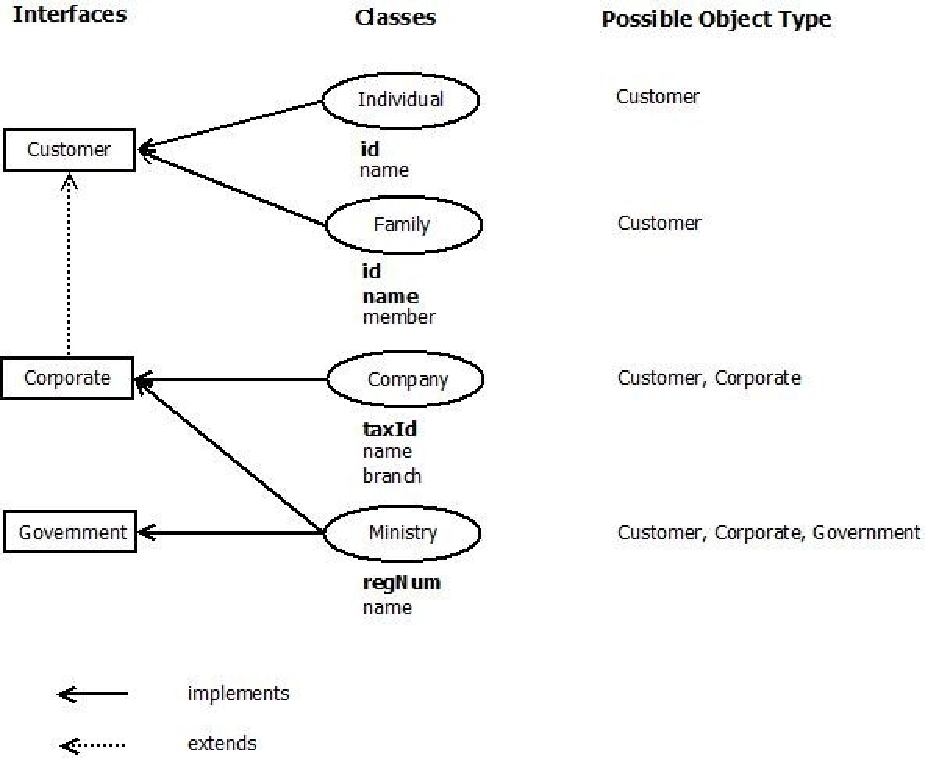
\includegraphics[scale=0.6]{sample.pdf}
	\caption{The Example of Retrieving Object Type}
	\label{figure1}
\end{figure}

\begin{figure}
	\centering
	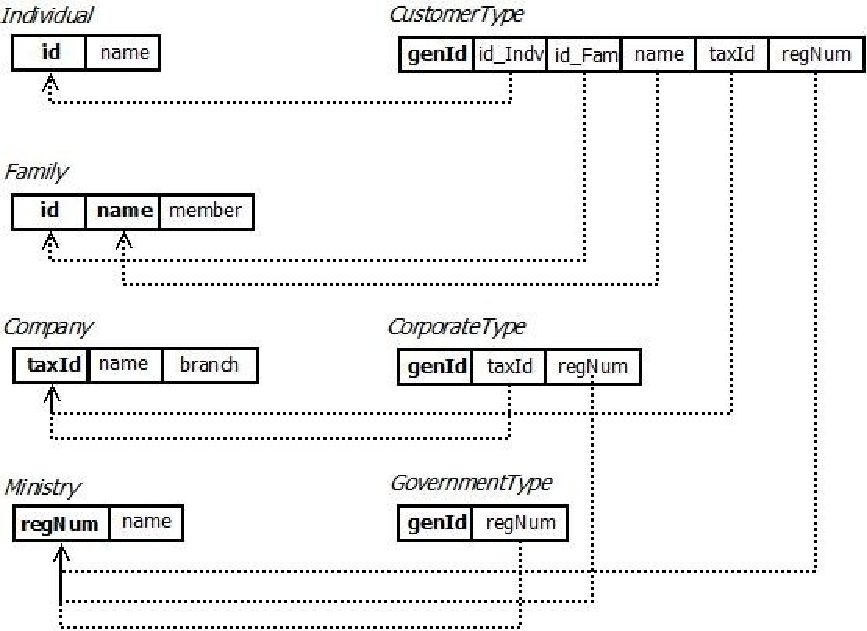
\includegraphics[scale=0.5]{db1.pdf}
	\caption{Database Schema Diagram}
	\label{figure2}
\end{figure}

\subsubsection{Referential Integrity in Relational Database}
There is another condition in ABS where the referential integrity constraint in relational database could be violated; that is when a class declaration has other objects as the class parameter or field. ABS, which is object-oriented, enables an object to have another object as its field. When a field is generated as the attribute in relational database, it is impossible to store the whole information of an object in an attribute. Hence, the solution is every time there is a class parameter or field declaration has interface type as the data type, the attribute generated will only contain the generated id of the object which is stored in the interface type table. This attribute will be the foreign key which refers to the primary key of the inference type table.

To describe the explanation above, we will use the same situation as the example beforehand. We add a new interface called Account. This interface is implemented by AccountImpl class. This additional situation is described by Figure 3 below.

\begin{figure}
	\centering
	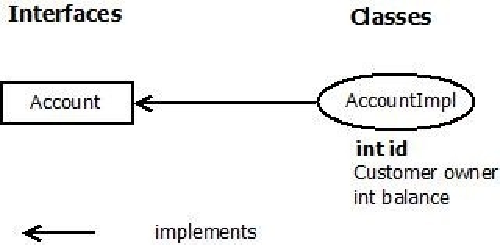
\includegraphics[scale=0.6]{sample2.pdf}
	\caption{Account Interface and AccountImpl Class}
	\label{figure3}
\end{figure}

Figure 4 presents the relational database schema based on the explanation above.

\begin{figure}
	\centering
	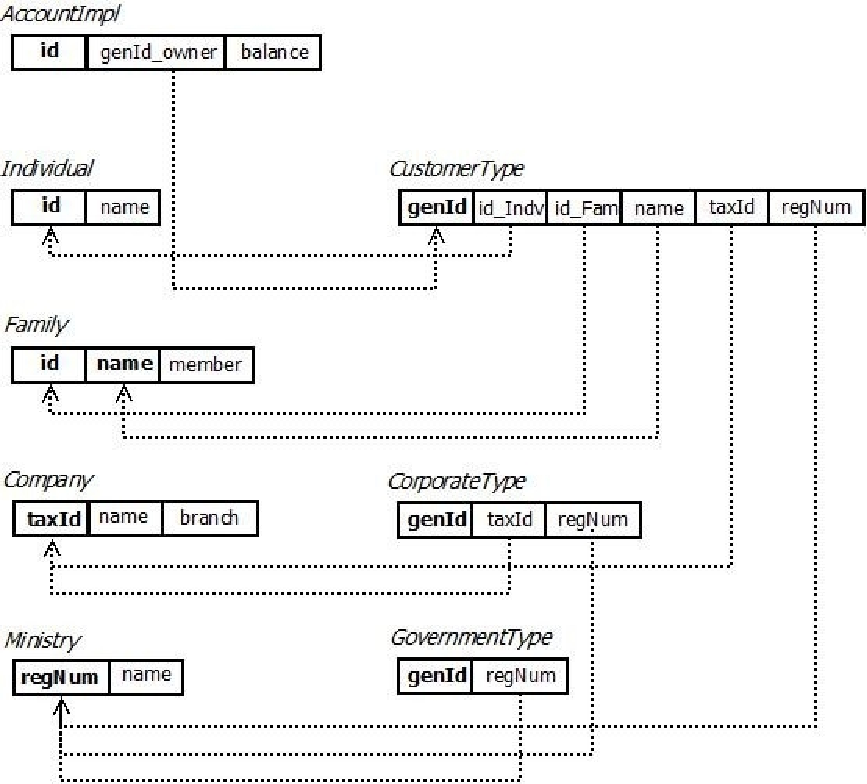
\includegraphics[scale=0.5]{db2.pdf}
	\caption{Database Schema Diagram with AccountImpl Class}
	\label{figure4}
\end{figure}


\section{Conclusion and Future Work}
This Section concludes the work and discusses about the future work.

\subsection{Conclusion}
Based on the goal of this research and the evaluation of case study in the previous section, we can conclude:

\begin{enumerate}
	\item Based on the results of this research, delta modeling in ABS can influence the elements of relational database schema.  The elements of relational database schema can be obtained from the core ABS, especially in the class declaration and interface declaration in every module. This base database schema, which is generated from the core ABS, can be affected by the implementation of delta modules. This case happens if the modification by the delta modules related to the class and the fields in a class.
	\item The mapping between ABS modeling and relational database schema is possible to be formulated, by considering the elements and the constraints owned by both sides. The elements which have similarities for both sides can be mapped directly. For example, an attribute of a class is mapped into attribute of a relation. However, there are several mismatches between both sides because of the conceptual differences. This can be solved by implementing some technique so that both sides’ constraints can be fulfilled. Using ABS annotations to declare primary key and generating intermediate table for object type are the solutions to the mismatches.
\end{enumerate}

\subsection{Future Work}
Basically this research is the first step of a bigger research that connects ABS to databases. Below is possible future work, which can be done to continue the process of connecting ABS to database.

\begin{enumerate}
	\item The normalization of the generated database schema to fulfill the normal forms in relational database schema.
	\item The implementation of the database operations: retrieval, deletion, and update. These operations will correspond to the method invocation in the main block of ABS. Moreover, this implementation relates to the ABS runtime.
	\item The usage of DBMS for database implementation in ABS: if DBMS will be used in database implementation by ABS, then the connection between ABS and DBMS must be formulated. An application program, in this case is ABS, accesses the database by sending queries or request for data in the DBMS. A query typically causes some data to be retrieved. A transaction done in application program may cause some data to be updated and written in the database. This connection will make ABS as a running application program which is able to access the database through the DBMS.
	\item Maintaining the evolvement of database connected to ABS because of the application requirement changes: requirement changes of application could lead to schema evolution where changes are needed to be applied to the schema. Moreover, this maintenance needs the consideration to preserve the previous data.
\end{enumerate}

\begin{thebibliography}{4}

	\bibitem{book1} Pohl, K., Bockle, G., Linden, F.J.V.D.: Software Product Line Engineering: Foundation, Principles and Techniques. Springer, New York (2005)

	\bibitem{book2} Elmasri, R., Navathe, S.B.: Fundamentals of Database Systems. Addison-Wesley, Boston (2011)

	\bibitem{lncschap} Reiner, Hahnle.: The Abstract Behavioral Specification Language. In: Giachino, E., Hahnle, R., Boer, F.S.D.B., Bonsangue, M.M. (eds.) Formal methods for Components and Objects. LNCS, vol. 7866, pp. 1-37. Springer, Heidelberg (2013)

	\bibitem{article} Khedri, N., Khosravi, R.: Handling Database Schema Variability in Software Product Lines. In: 2013 20th Asia-Pacific Software Engineering Conference(ASPEC), pp.
	3311-338. IEEE Computer Society, California (2013)

\end{thebibliography}

\end{document}


